%% CORREGIR %%%%

%%%%%%%%%% NO OLVIDAR COLOCAR ESTE COMENTARIO CON EL NUMERO DE EJERCICIO %%%%%%%%%%%%%
%%%%%%%%%%%%%%%%%%% EJERCICIO 1 %%%%%%
%%Text bf para negrilla , el \\ es para el salto de linea.
%%El primer \\ hace un espacio en el  texto y el 2 \\ crea otro espacio
\textbf{Ejemplo 1}\newline
Se necesita adquirir un motor para la planta de acabados de una fábrica, en el mercado existen dos marcas de motores que cumplen con las especificaciones técnicas de potencia, velocidad, eficiencia, etc.
La información que desde el punto de vista económico se proporciona, es la siguiente:\\ 
\begin{center}
		\begin{tabular}{|c|c|c|c|}
			
			\hline
			\rowcolor[HTML]{FFB183}
			  &                               & A       & B       \\ \hline
			1. & Costo inicial (P)                 & 100.000 COP & 500.000 COP \\ \hline
			2. & Costo mensual de operación ($R_m$)   & 5.000 COP   & 10.000 COP \\ \hline
			3. & Años de vida útil (n)            & 5       & 20      \\ \hline
			4. & Valor de salvamento (VS)           & 15.000 COP  & 150.000 COP \\ \hline
			5. & Reparación general del año 12 ($R_{rep}$) & -      & 200.000 COP \\ \hline
		\end{tabular}
  \hspace{1cm}
\end{center}

Con una tasa del 2.5 nominal anual mes vencido, hallar la mejor alternativa. \\

\textbf{Solución.}\\



\begin{center}

	\renewcommand{\arraystretch}{1.5}% Margenes de las celdas
	%Creación de la cuadricula
	\begin{longtable}[H]{|c|c|c|}
		%Creamos una linea horizontal
		\hline
		%Definimos el color de la primera fila
		\rowcolor[HTML]{FFB183}
		%%%%% INICIO ASIGNACIÓN FECHA FOCAL %%%%%%%
		%%%%%%%%%% INICIO TITULO
		%Lo que se hace aquí es mezclar las 3 columnas en una sola
		\multicolumn{3}{|c|}{\cellcolor[HTML]{FFB183}\textbf{1. Asignación período focal}}   \\ \hline
		%%%%%%%%%% FIN TITULO
		%%%%% INICIO DECLARACIÓN DE VARIABLES %%%%%%%
		\multicolumn{3}{|c|}{$pf : 0 pav$} \\ \hline
		%Definimos el color de la primera fila
		
		%%%%% INICIO DECLARACIÓN DE VARIABLES %%%%%%%
		%%%%%%%%%% INICIO TITULO
		\multicolumn{3}{|c|}{\cellcolor[HTML]{FFB183}\textbf{2. Declaración de variables}}\\ \hline                                                      %%%%%%%%%% INICIO SUBTITULO
    \cellcolor[HTML]{FFB183}\textbf{Variables monetarias}    & 
    \cellcolor[HTML]{FFB183}\textbf{Variables conceptuales} &
    \cellcolor[HTML]{FFB183}\textbf{Incógnitas}  \\ \hline
    %%%%%%%%%% FIN SUBTITULO                            
		%%%%%%%%%% FIN TITULO
		%%%%%%%%%% INICIO DE MATEMÁTICAS
    
    % Valores monetarios para Alternativa A y B
    \multicolumn{1}{|c|}{$P_A = 100{.}000\text{ COP}$} & \multicolumn{1}{c|}{$n_A =  5 \textit{ años }$} & \multicolumn{1}{c|}{$CAUE_{A} =  \text{? COP}$}\\
    \multicolumn{1}{|c|}{$VS_A =  15{.}000\text{ COP}$} & \multicolumn{1}{c|}{$n_B =  20 \textit{ años }$} & \multicolumn{1}{c|}{$CAUE_{B} =  \text{? COP}$}\\
    \multicolumn{1}{|c|}{$R_{mA} = 5{.}000\text{ COP}$} & \multicolumn{1}{c|}{}  & \multicolumn{1}{c|}{}\\
    \multicolumn{1}{|c|}{$P_B = 500{.}000\text{ COP}$} & \multicolumn{1}{c|}{$i= 2,5\% \textit{ pmv } \equiv 34,489\% \textit{ pav}$}& \multicolumn{1}{c|}{}\\
    \multicolumn{1}{|c|}{$VS_B =  150{.}000\text{ COP}$}& \multicolumn{1}{c|}{} & \multicolumn{1}{c|}{}\\
    \multicolumn{1}{|c|}{$R_{mB} = 10{.}000\text{ COP}$}& \multicolumn{1}{c|}{}& \multicolumn{1}{c|}{}\\
    \multicolumn{1}{|c|}{$R_{rep} = 200{.}000\text{ COP}$}& \multicolumn{1}{c|}{}& \multicolumn{1}{c|}{}\\\hline


		%%%%% INICIO FLUJO DE CAJA
		\rowcolor[HTML]{FFB183}
		\multicolumn{3}{|c|}{\cellcolor[HTML]{FFB183}\textbf{3. Diagrama de flujo de caja}}                                                                                  \\ \hline
		%Mezclamos 3 columnas y pondremos el dibujo
		%%%%%%%%%%%%% INSERCIÓN DE LA IMAGEN
		
		\multicolumn{3}{|c|}{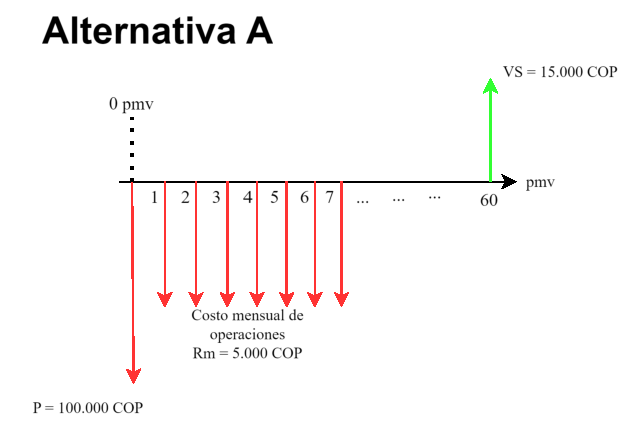
\includegraphics[trim=-5 -5 -5 -5, width=10.5cm, keepaspectratio]{10_Capitulo/img/ejemplos/PDFs/1/Ejemplo_1_A.pdf}}\\ \hline
		\multicolumn{3}{|c|}{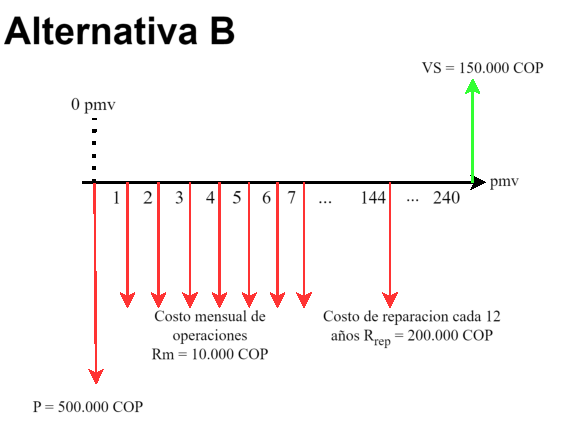
\includegraphics[trim=-5 -5 -5 -5, width=10.5cm, keepaspectratio]{10_Capitulo/img/ejemplos/PDFs/1/Ejemplo_1_B.pdf}}\\ \hline
		%%%%%%%%%%%%% FIN INSERCIÓN DE IMAGEN
		%%%%%FIN FLUJO DE CAJA



		%%%%% INICIO DECLARACIÓN FORMULAS
		%%%%%%%%%%% INICIO TITULO
		\rowcolor[HTML]{FFB183}
		\multicolumn{3}{|c|}{\cellcolor[HTML]{FFB183}\textbf{4. Declaración de fórmulas}}                                                                                    \\ \hline
		%%%%%%%%%%% FIN TITULO
		%%%%%%%%%%% INICIO MATEMÁTICAS

		\multicolumn{3}{|c|}{$VP=R\frac{1-(1+i)^{-n}}{i} \text{ Valor presente serie uniforme vencida}$}\\ 
		\multicolumn{3}{|c|}{$VF=R\frac{(1+i)^{n}-1}{i} \text{ Valor futuro serie uniforme vencida}$}\\
		\multicolumn{3}{|c|}{$CAUE = \sum Ingresos_{anualizados} - \sum Egresos_{anualizados} \text{ CAUE expresado como una sumatoria}$}\\
		\hline
		%%%%%%%%%% FIN MATEMÁTICAS
		%%%%%% INICIO DESARROLLO MATEMÁTICO
		\rowcolor[HTML]{FFB183}
		%%%%%%%%%%INICIO TITULO
		\multicolumn{3}{|c|}{\cellcolor[HTML]{FFB183}\textbf{5. Desarrollo matemático}}                                                                                      \\ \hline
		%%%%%%%%%% FIN TITULO
		%%%%%%%%%% INICIO MATEMÁTICAS
        Alternativa A & \multicolumn{2}{c|}{Alternativa B} \\ \hline
        
		Pasar el costo de operacion de $R_m$ a $R_a$: & \multicolumn{2}{c|}{Pago año 12 ($R_{rep}$) en valor presente} \\
  
		$R_a = {5{.}000*\frac{(1+0,025)^{12}-1}{0,025} = 68{.}978 COP}$ & \multicolumn{2}{c|}{${VP=200	{.}000(1 + 0,34489)^{-12} =  5{.}712}COP$}\\
  
        $ $  & \multicolumn{2}{c|}{}\\
        
		Dividir los 100.000 en 5 pagos anuales uniformes: & \multicolumn{2}{c|} {Nuevo P}\\
  
		${R_1={100{.}000} * \frac{0,34489}{1-(1+0,34489)^{-5}} = 44{.}633}COP $  & \multicolumn{2}{c|}{P = $500{.}000COP + 5{.}712COP = 505{.}712COP$}\\

        $ $  & \multicolumn{2}{c|}{}\\
  
		Dividir los 15.000 en 5 pagos anuales uniformes &\multicolumn{2}{c|} {dividir los 505.712 en 20 pagos anuales}\\
  
		$R_2={15{.}000}* \frac{0,34489}{(1+0,34489)^{5}-1} = 1{.}522COP $ & \multicolumn{2}{c|}{${R_1={505{.}712} * \frac{0,34489}{1-(1+0,34489)^{-5}} = 174{.}882 }COP$}  \\ 

        $ $  & \multicolumn{2}{c|}{}\\
  
		CAUE alternativa A &\multicolumn{2}{c|}{Cuota anual valor salvamento}\\ 
		$CAUE_{A} = 1.522-44.633-68.978$ &\multicolumn{2}{c|}{${R_2={150{.}000}* \frac{0,34489}{(1+0,34489)^{20}-1} = 138COP }$}\\ 

        $ $  & \multicolumn{2}{c|}{}\\
  
		$CAUE_{A} = -112.089 COP$ &\multicolumn{2}{c|}{Pasar el costo de operacion de $R_m$ a $R_a$}\\ 
		&\multicolumn{2}{c|}{$R_a = {10{.}000*\frac{1,025^{12}-1}{0,025} = 137{.}956 }COP$} \\ 

        $ $  & \multicolumn{2}{c|}{}\\
  
		& \multicolumn{2}{c|}{CAUE alternativa B} \\ 
		&\multicolumn{2}{c|}{$CAUE_{B} = 138-174.882-137.956$}\\ 
		&\multicolumn{2}{c|}{$CAUE_{B} = -312.700COP$} \\ \hline
		%%%%%%%%%% FIN MATEMÁTICAS
		%%%%%% FIN DESARROLLO MATEMÁTICO

		\rowcolor[HTML]{FFB183}
		\multicolumn{3}{|c|}{\cellcolor[HTML]{FFB183}\textbf{6. Respuesta}}    \\ \hline

		\multicolumn{3}{|c|}{La alternativa que representa menores perdidas es la A.} \\ \hline
	\end{longtable}
	%Se crean dos lineas en blanco para que no quede el siguiente texto tan pegado
	%\newline \newline
\end{center}
%%%%%%%%%%%%%%%%%%%%%%%%%%FIN EJERCICIO X %%%%%%%%%%%%%%%%%%%%%%%%%%%